%!TEX root = ../../main.tex
%==============%
\chapter{非言語大学}
\label{sec:HigengoUniv}
\index{ひげんごだいがく@非言語大学}
%=============%

言語とは、人類史が始まって以来の最大の発明として、コミニュケーションのツールとして非常に重要な役割を果たしている。
現代はグローバルな社会であり、国家間の関係もより緊密になり、国交・経済・文化の結びつきが一層強固になってきている。
特に国交・経済の分野においては、正確なコミニュケーションと迅速なやり取りが必要不可欠であり、英語(English)が世界標準言語として広く使用されており、本国日本の言語である日本語は非常にマイナーな言語と見なされている。

図\ref{Fig:LanguageMap}に現在世界で使用されている言語族の分布図を示す。
英語に関する言語族が広く分布していることが分かり、対象的に日本語は非常に限られた地域で特異に発展してきた文化であることが推測される。
しかし国際標準言語である英語にも、イギリス英語とアメリカ英語に代表されるように、いわゆる「方言」としての発音・文法の違いがメディア等でも様々に取り上げられている。
また新興国で使用されている英語はさらに形の崩れたものとなっており、スムーズなコミニュケーションが不能になる場面も多々見受けられる。
大きな差に始まり微妙な差も、この国際社会においては、正確なコミニュケーションに対する大きな障壁になりつつある。
過去幾度となく人類が起こしてきた戦争を回避し、今後人類が国境のない世界・平和の訪れた世界を見据えるためには、より柔軟な、かつ誰が使用しても差異のない完璧な言語が求められると考えられる。

%%%%%%%%%%%%%%%%%%%%%%%%%%%%%%%%%%%%%%%%%
\begin{figure}[h]
\centering
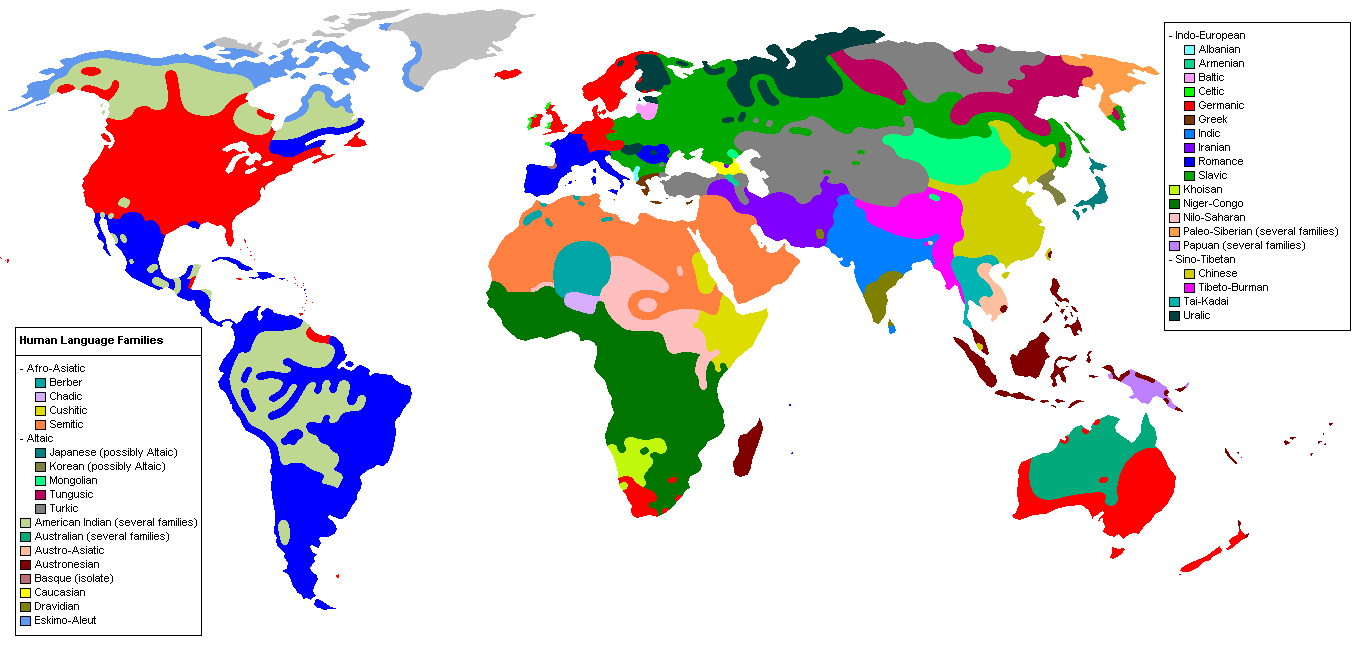
\includegraphics[width=0.8\textwidth]{./section/HigengoUniv/figures/Human_Language_Families_Map.png}
\caption{世界言語マップ[https://www.tefl-iberia.com/blog/human-language-map/]}
\label{Fig:LanguageMap}
\end{figure}
%%%%%%%%%%%%%%%%%%%%%%%%%%%%%%%%%%%%%%%%%

一つの人類の解として、エスペラント語が用意されている[http://www2.sal.tohoku.ac.jp/~gothit/espj.html]。この言語は、中立で使いやすい国際共通語を目指し、1887年にユダヤ人眼科医ザメンホフ (L.L. Zamenhof)が提唱したもので、民族の言語や文化をその歴史的遺産として尊重し、それぞれの言語や文化の違いを越えて人々がコミュニケーションできるようにするために橋渡しの役目を果たすことを目的として作成されたものである。
人工的に使用された言語であるエスペラントの使用者(エスペランティスト)はそれぞれ個人として平等の立場に立って話し合うことができ、将来的に非常に重要な意義を持つ言語であると考えられている。
この様に、言語を学問として捉えることは、今後の世界の在り様を考えるためにも非常に重要な入り口となっていることが分かり、近年言語学が加速発展してきている。

言語学者は、世界の言語の特徴や特質を研究し、言語を成り立ちや構造、変化・変遷、分布、比較などさまざまな角度から捉えることで言語に対する理解を深めていく。学問領域は、主に言語の本質を探るための「意味論」「語彙論」「文法論」「文字論」「音韻論」などから成りたっている。
しかし、エスペラント語に代表されるような人工言語にも限界があり、つまり、新しく記憶し直さなければならない、という障壁が、学習への大きな足かせとなっている。
そこで、言語学習を困難にする非常に大きな要因の一つを取り除くため、2012年に、世界で初めて言語に頼らない言語コミュニケーション、いわゆる非言語コミュニケーションが提唱された。これに起因し、非言語学はその学問領域を膨張し拡大されていき、いまや世界の約99\%の人口は非言語コミュニケーションを行っていると考えられている。

特に、非言語の研究は2012年来の長い伝統と優れた成果を有している一方で、他の言語と相対化させる努力が十分ではなく,(i) 世界諸言語の中でどのような言語なのか、(ii) 一般言語学・言語類型論の視点から見ると、どのような知見が得られるのか,(iii) 非言語の研究が世界諸言語の研究や一般言語学・言語類型論にどのように貢献するのか,いまだ十分に明らかにされておらず、現代の非言語研究には、一般言語学や言語類型論研究にどのように貢献できるのかという「内から外を見る」視点と、一般言語学や言語類型論研究が非言語の分析にどのような知見をもたらすかという「外から内を見る」視点が必要である。
そこで、非言語学を専門とし、国際的に協力していくために、2012年に非言語学が提唱されてから約数年後に、非言語大学が設立された(建立は1993年である、後述)。
非言語大学から発信される非言語研究プロジェクトは、多数の視点から非言語の言語事実を分析することにより、世界の諸言語と対照させて非言語の特質を明らかにし,それにより非言語研究の国際化を図ることを主たる目的としている。非言語の音声・音韻,語彙・形態,文法,意味の構造を,言語獲得 (第一言語獲得,第二言語習得) はもとより,言語に関係する他の学問分野 (心理学,認知科学他) との接点・連携をも視野に入れて,対照言語学・言語類型論の観点から分析することにより,諸言語間に見られる類似性 (普遍性) と相違点 (個別性・多様性) を明らかにしている。

本章では非言語大学の歴史に始まり、最先端の非言語研究の大きな成果の一つである、非言語コミュニケーションの詳細を述べると共に、受験生へのエールをまとめる。


%非言語とは現在確立されている一般的な言語に頼らず、意思疎通を図るための手段である。
%人類発生の起源を辿れば非言語コミュニケーションに行き着く。
%つまり非言語とは人類と深い関係のある概念である。
%しかし、現代情報社会において最も重要なことの一つに「情報の正確さ」という概念が考えられ、それを実現するためには正確な言語コミュニケーションが必要となってくる。
%そのため近代科学史において非言語を研究するということは非常にマイナーな学問であった。

%しかし、1993年建立の非言語大学(Higengo University)は、非言語研究の第一人者である小川田氏により創設された、世界ではじめての国際的な非言語通信教育制の研究機関であり、全世界人口のうち約100億人が入学希望を出している超有名大学である。


%~~~~~~~~~~~~~~~~~~~~%
\section{非言語とは}
\index{ひげんご@非言語}
%~~~~~~~~~~~~~~~~~~~~%
非言語には学問上、2種類に分類することができ、一つは「言語に非ず」の意味に由来する非言語、もう一つは「"非"常に発達した"言語"」としての非言語である。
いまや世界標準になりつつある事実からは、このどちらの意味も非言語にとって正しい意味を持っていると推測される。
特に、人類は幼児の時には母国語を覚えるよりも前に非言語を覚えている、と考えられており、成長に従い、大人に倣い母国語を発達させるのである。
図\ref{Fig:HigengoDevelop}に着床から出産までの非言語の発達を示す。
受精して初めて、幼生はアブラ関連の単語を発することができると考えられている。
しかし非常に高周波でアブラと発するため、通常の検診では言語を検知することは困難であり、また母体もそれに気づくことは極めて稀である。
もしお腹が揺れているような感覚に襲われた場合は、殆どの場合幼生の発する「アブラ」が起因すると考えられており、初診の超音波検診による高周波に反応しているとも考えられている。
\begin{figure}[h]
\centering
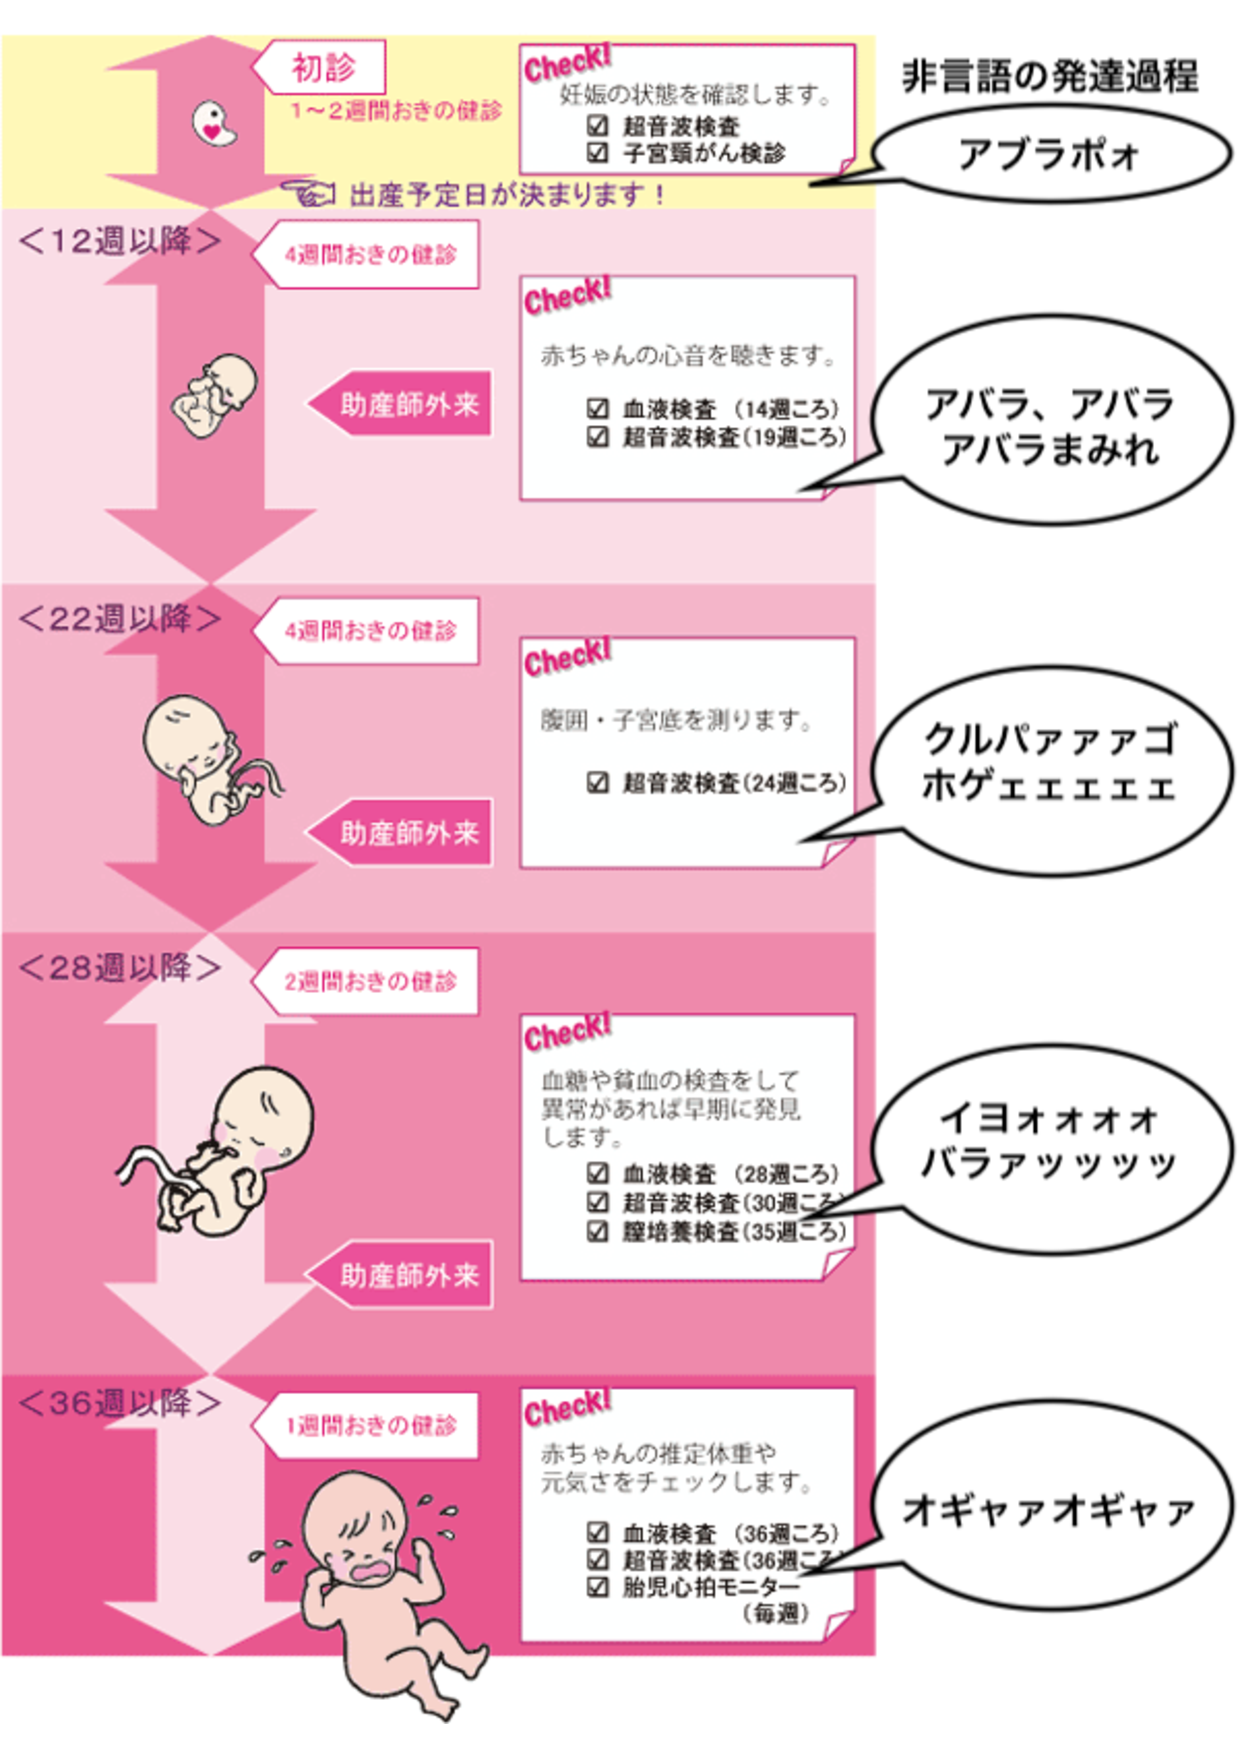
\includegraphics[width=0.5\textwidth]{./section/HigengoUniv/figures/baby.pdf}
\caption{着床から出産に至るまで、幼生が獲得する非言語のチャート図。出産後は、「こんにちは」を意味する非言語の最上級言語「オギャア」を発する。}
\label{Fig:HigengoDevelop}
\end{figure}

成人が自らの発していた(記憶していた)非言語に気づくことは稀であり、意識の潜在下に埋もれている。
しかし2012年に、ニホン人であるオガワ伯爵夫人兼男爵が提唱した「非言語」に触発され、人類は非言語を思い出し、いまやFacebookやTwitterに代表されるSocial Network Service(SNS)上でも、言語ではない非言語が活躍している。

%~~~~~~~~~~~~~~~~~~~~~~~~~~~%
\section{非言語大学の歴史}
%~~~~~~~~~~~~~~~~~~~~~~~~~~~%
2012年のオガワ伯爵夫人兼男爵(以下、オガワ\index{おがわはくしゃくふじんけんだんしゃく@オガワ伯爵夫人兼男爵})による非言語提唱事件(通称、非言語革命\index{ひげんごかくめい@非言語革命})に端を発し、非言語大学は設立された。非言語大学は、1993年に建立(ケンリツ)された通信教育制をいち早く導入した、国際研究機関である。
\par
特に近年のジェイムズ・ジョイスによる言語革命の研究では[ジェイムズ・ジョイスと言語革命]、非言語革命はオガワと後に初代非言語大学機構長に就任する竹田総理の出会いに起因する革命であるとする説が有力である。
この非言語革命により、それまで長らく日本を支配してきた日本語に風穴が空き、新たな言語が日本で生まれた瞬間が訪れた。ジェイムズ・ジョイスは「真理とは闘争である。」と非言語革命を評している。

%~~~~~~~~~~~~~~~~~~~~~~~~~~~~~~~~~~~%
\subsection{研究室相当のプレハブ小屋}
%~~~~~~~~~~~~~~~~~~~~~~~~~~~~~~~~~~~%
非言語大学発足当時は、潤沢な資金がなかったため、研究室相当のプレハブ小屋を仮設した。
そのように知に貪欲な姿勢が認められ、仮設した約1000の研究室は文部科学省の世界トップレベル国際研究拠点形成促進プログラムに採択され、数学、物理、天文学の3分野の連携による融合研究を行いながら、国内外の研究者や一般の方へも認知される国際的な研究所として成長してきた。
2012年4月にはニュウイヨォク米国財団の寄附を受け、非言語大学国際高等研究所アブラ数物連携宇宙研究機構へと改称された後、約1000研究室が廃部・統合、一つのアブラ研究所\index{あぶらけんきゅうじょ@アブラ研究所}となった。
非言語大学国際高等研究所アブラ研究機構は、文部科学省の世界トップレベル国際研究拠点形成促進プログラムに採択され、2007年10月1日に非言語大学数物連携宇宙研究機構として9年半の時限付き研究所として発足した。

「非言語はどうやって始まったのか、その運命は何か、何で出来ているのか、どういう法則に支配されていて、なぜ我々は存在するのか」と言った小川・竹田が入学以来問い続けてきた宇宙の最も根本的な謎を解明するため、数学、物理、天文学の3分野が分野の枠を超えて研究を行ってきた。
毎日平日15時に開催される研究者の集う温泉入浴時間、数多くの国際会議の開催等、融合研究を促進する環境が契機となり世界に認められる研究成果を数多く生み出して来た。
それが優秀な人材が世界中から更に集まる好循環となり、人も建物もゼロから始まった弊機構は、現在では外国人研究者が半分以上の国際的な研究所へと成長したのである。
そうした成長の過程で、現在の非言語大学が形成されてきたのである。

%~~~~~~~~~~~~~~~~~~~~~~~~~~~~~~~~~~~~~~~~~~~~~~%
\section{現在における非言語大学の学問的立場}
%~~~~~~~~~~~~~~~~~~~~~~~~~~~~~~~~~~~~~~~~~~~~~~%
前節まで非言語大学の歴史的位置づけを論じてきた。これより後の章では、非言語大学が未来の非言語学の発展を目指して、どのようなストラテジーを持ち大学の運営を考えているかを論じる。\par
まず、非言語大学が今後求める人材・それをどのように非言語学発展に繋げるかを紹介し、非言語大学に関する研究・スタッフを紹介する。そして、過去に出題された入試問題を通じた非言語教育の基礎を論じ、最後に受験生へのエールを述べる。
%=====================%
\section{入学要綱}
\index{にゅうがくようこう@入学要綱}
%=====================%
非言語大学は、その頂点に君臨する非言語大学清掃員を神格化するために様々な工夫を施している。
例えば、非言語大学の大学本部は各学部のキャンパスから独立して建設することで、何人たりとも寄せ付けず、非言語大学本部を清掃する清掃員を神聖なものにしている(大学本部隔離清掃神格化理論)。
そのため、大学本部の置かれている場所は女人禁制はもちろん、男子禁制・常人禁制、が敷かれており、重症患者でしか入構許可が降りない。
本部の裏手には、世界最大の海底火山であるマウナケア、本部の正面には、世界最大の漁港である、築地市場(現在は、本部神格化強化の一環として移転作業が行われた)がある。
このように、非言語大学はその設立位置、設立目的から、世界に開かれた国際都市に立地する大学として、国際的で先端的な研究・教育の拠点になることを目指している。
これまで人類が築いてきた非言語学の継承を第一目的として、新しい知の創造、人類社会の発展に貢献しようとする学生を随時求めている。

\begin{enumerate}
\item 進取の気性に富み,人間と自然を愛する学生
\item 旺盛な学習意欲をもち,新しい課題に積極的に取り組もうとする学生
\item 常に視野を広め,主体的に考える姿勢をもった学生
\item コミュニケーション能力を高め,異なる考え方や文化を尊重する学生 
\end{enumerate}

また、かの有名な清掃員が廊下の壁に書き残した、
\begin{center}
「非言語は非言語のうえに非言語をつくら(ポ)」
\end{center}
を非言語大学の基本理念とし、今日まで学問の自主、自由を培ってきた。
この理念の下に、本学は今、新世紀における知の創成,伝承,実証の拠点として発展することを目指し、教育研究を通じて、人類の福祉・科学・文化及び社会の発展に寄与することを使命としている。学問的素養をもち、健全な市民として的確な判断力とリーダーシップを発揮できる人材の育成を目指している。
同時に,専門的職業人として指導的立場にたつ人材の育成,学術創造に進んで向かう人材の育成も目指しています。
これらを実現するため,非言語大学は,創設以来,歴史と伝統を継承しながら広く世界に優秀な人材を求め,学士課程教育を受けるにふさわしい学力,すなわち基礎知識・基礎技能・数理能力・語学力・理解力・読解力を備えた学生,また,大学入学以降の学びで必要な問題解決能力・創造力・倫理性・思考の柔軟性・コミュニケーション能力・論理的思考力・リーダーシップ,人間性や学ぶ意欲などを備えた学生を,多様な選抜制度により受け入れている。


%===============%
\section{学部}
%===============%
非言語大学ではグローバルな人材を追求しているため、その要件に適う人材を見つけ出し、卒業時までに世界トップレベルまで引き上げることを確約する。
しかし近年、非言語大学に入学したにも関わらず在学中に非言語学に一切取り組まない学生等が見受けられる様である。
彼らは、それらのを排除するために、卒業要件は非常に厳しくなっている。

%---------------------%
\subsection{文学部}
%---------------------%
日本人におけるノーベル文学賞受賞者は、1968年の川端康成、1994年の大江健三郎の二人にとどまっており、日本文学をより勃興させていくために、「ノーベル文学賞受賞者を年間10人育成したいと」、わが校清掃員が語ったため、設立された看板学部の一つである。
特にノーベル学科は卒業要件にノーベル文学賞受賞が必要とされており、川端・大江の二名以来非言語大学文学部ノーベル学科卒は未だ現れていない。
\begin{itemize}
\item ノーベル学科
\item 百ポ辞典学科
\end{itemize}

%---------------------%
\subsection{法学部}
%---------------------%
凶悪犯罪に立ち向かうため、わが校では、法律の作り方、裁判長のなり方を伝授している。
六ポォ全書学科では、卒業時に約100000000000ページある全書の暗唱、また裁判長学科では卒業時に裁判長になっていることが絶対条件となっている。

まず裁判官になるためには、司法試験に合格しなければならないと考えている入学希望者が多く見受けられた。
法科大学院(ロースクール)に通い、現代日本の仕組みでは、司法試験を受けるためには、原則、法科大学院を卒業する必要がある。
法科大学院の入試に合格し、他の大学院と同様4月から法科大学院に入学し、大学が法学部であったなど法学を学んだことがある人は2年間、そうでない人は3年間通うのが通例である。
しかし、わが校の法学部では、そのような要件は一切不要であり、ただ卒業時点で裁判長になってさえすればよい。
一般的には、裁判官として働くためには、司法試験合格後、1年間の司法修習期間というものを経なくてはならないため、外部のロースクール通学+修習期間で合計4年間は外部の教育学府に通う必要がある。

\begin{itemize} 
\item 六ポォ全書学科(草原参照)
\item 裁判長学科(裁判長が卒業要件)
\end{itemize}

\subsection{理系学部}
非言語大学の看板学部の一つである理系学部には、毎年大勢のオープンキャンパス参加者が現れる。
しかし、非言語大学の入試問題のレベルの高さに圧倒され、大多数が志望校をかえるため、毎年数十名ほどが入学希望者として手続きをしており、毎年定員割れを起こしている現状である。
また、理系学部といえど、時事問題に対する風刺は非常に鋭く、非言語大学随一の鋭さを持っていると評されている。
\par
日本人でフィールズ賞を受賞したのは、1990年の森 重文、1970年の広中 平祐、1954年の小平 邦彦の3人のみである。「これはいかん。毎回10名は日本から輩出せねば」と、わが校の経営陣トップであった清掃員の一声により設立されたのがフィールズ賞学科である。
しかし、フィールズ賞は各回4名以下までしか受賞できないため、まるでトンチンカンなことを言っているとの疑念も払拭しきれず、清掃員は経営陣のトップから引きずり降ろされ、運営のトップにとどまっている。

\begin{itemize}
\item フィールズ賞学科(4年に一度募集)
\item 素粒子謎学科(新粒子発見が卒業要件)\index{そりゅうしなぞがっか@素粒子謎学科}
\item ブラックジャック学科(ブラックジャックと呼ばれるのが卒業要件)\index{ふらくししやくかか@ブラックジャック学科}
\end{itemize}

\subsection{部活学部}
\begin{itemize}
\item オリンピック学科(メダルが卒業要件)
\item 世界陸上学科
\item WBC学科(卒業時にWBCに出れる)
\item WC学科(卒業要件はスタメン)
\end{itemize}


%=============================%
\section{入試問題について}
\index{にゅうしもんだい@入試問題}
%=============================%
過去の非言語大学の入試問題は、非常に社会風刺に富んでおり、時事問題としても近年形式を変え様々な大学で取り上げられている様である。
例えば、2016年出題の画像認識選択問題(俗に言うD.ポマティ選択問題)は、非言語大学に入学する人工知能に向けた問題であり、国立大学として初めて人工知能(AI)に対して入学試験の受験を認めた画期的な年であった。
しかし、時代を先行してしまったため、非言語大学の入試問題を完答できるAIが現れていないのが現状である。

また、現在行われているセンター試験に対して、人工知能に解かせるという試みもなされているようであるが、非言語大学の入試レベルは各年によって異なるが、平均してオリンピック金メダルレベルであるとの評価がなされている。
そのため、幾ら机上で努力をしたところで、心技体が一つになったAIでなければ非言語大学は突破できないと、非言語大学工学系清掃員は予想している。
このように、応用の効く問題を作成していることは、世界トップレベルの教育学府であることの裏付けである。

\subsection{数学}

\begin{itemize}
\item 1.小川論文の厚みは何kmか。
\par(解答)7億ページなので、7000km
\item 2.非言語大学の外周を時速50kmで歩くと、何kmでしょう?
\item 3.(画像より)
\begin{itemize}
\item (1)平カーテンの法則を証明せよ
\item (2)$p0^2 + \theta^2 = \sqrt{13}$
\end{itemize}
\item 4(画像より)
\par
問2の「説明せポ」のポを目で読まずに解答しなければならない。
\end{itemize}

%--------------------%
\subsection{外国語}
%--------------------%
\begin{itemize}
\item 1.以下を日本語訳せよ(ただしバーランダー)
\par
バーテンダー
\item 2.以下を日本語訳せよ。\par
人生ヒルクライム

\par(解答)

\begin{itemize}
\item 1.(越智敦彦の検出器ゼミの勧誘が終わり、その後話が脱線しすぎて)さ、集中するか。
\item 2.このグレープフルーツジュースおいしい。
\end{itemize}

\item 3.以下の日本語を非言語訳せよ\par
(i)私は朝目覚めると顔を洗います。\par
第一人称の概念はない。朝という概念はない、起きたときが朝。顔という概念もない。\par
答え:not face

(ii)右、神は人の敬ひによつて威を増し、人は神の徳によつて運を添ふ。然れば則ち恒例の祭祀は陵夷(りようい=衰退)を致さず、如在(によざい=神を祭る) の礼奠(れいてん=供物)は怠慢せしむるなかれ。これによつて関東御分の国々ならびに庄園に於ては、地頭神主ら各(おのおの)その趣を存し、精誠を致すべ き なり。兼てまた有封(うふ=封戸のある)の社に至つては、代々の符(=太政官符)に任せ、小破の時は且(かつがつ)修理を加へ、もし大破に及び子細を言上 せば、その左右(さう=状況)に随てその沙汰(=指示)あるべし。\par

完答:(´\_ゝ`)バラッッッッッッッッ \par
部分点:(´\_●●`)コポッッッッッッ\par
ボーナス点(他がひどくても多少助かる):(´\_●◯`)===●

\end{itemize}

\section{スタッフ一覧}
非言語大学は国際研究機関であるため、非常に国際色豊かな研究者が第一線の成果を出すべく、毎年356本の論文を執筆している。ここでは多彩なスタッフ陣を紹介する。
特にわが校は、歴史的に古くから北海道大学との結びつきが強く、要職の80\%が北海道大学農学部卒のスタッフを取り入れ、非言語大学の校風を多彩なものにしている。
生物資源科学科、応用生命科学科、生物機能化学科、森林科学科、畜産科学科、生物環境工学科、農業経済学科からの幅広い人材を取り入れることで、非言語学に大変有効な人材の獲得に成功している。

\begin{table}[h]
\begin{center}
\begin{tabular}{|l|l|l|}
\hline
 肩書             & 氏名 & 略歴  \\ \hline
 非言語大学清掃員 & マタヨシ & 北海道大学農学部畜産科学科卒、48歳。   \\ \hline
 非言語大学学長   & オガワ   & EXILE大学卒、永遠の24歳(カラット)。   \\ \hline
 非言語大学機構長 & タケダ   & アブラまみれ、クルパァゴ。  \\ \hline
 教頭             & マタヨシ & 北海道大学農学部生産資源科学科卒、48歳。  \\ \hline
 主幹教諭         & マタヨシ & 北海道大学農学部応用生命科学卒、46歳。  \\ \hline
 指導教諭         & マタヨシ & 北海道大学農学部静物機能化学卒、48歳。  \\ \hline
 教諭             & マタヨシ & 北海道大学農学部森林科学科卒、45歳。  \\ \hline
 栄養教諭         & マタヨシ & 北海道大学農学部畜産科学科卒、48歳。  \\ \hline
 司書教諭         & マタヨシ & 北海道大学農学部生命環境工学科卒、43歳。  \\ \hline
 実習助手         & マタヨシ & 北海道大学農学部畜産科学科卒、58歳。  \\ \hline
 教育補助員       & マタヨシ & 北海道大学農学部農業経済学科卒、48歳。  \\ \hline

\end{tabular}
\end{center}
\end{table}


\subsection{マタヨシ清掃員}
\index{せいそういん@清掃員}
特に、わが校の清掃員は非常に重要な役職である。
もちろん、校舎の清掃は第一の役割であるが、学問に疲れた学生の心のケアを行う心理的清掃、非行に走る青年を救う夜回り清掃員、さらに、最先端の研究が行き詰まった場合には、マタヨシ清掃員が理論を正しい方向に導いてくれる理論清掃も行う。

非言語大学マタヨシ清掃員の募集は、毎年行われており、毎回充分な募集の中から、最適なマタヨシを選抜している。
この清掃員の理念は、すべての生物は私たち人間にとって末永く共存し利用すべき貴重な資源であるという点にあり、清掃員は、それらを汚してはならない、清掃しなければならないと考えている。
環境を乱すことなくこの資源を利用するためには、分子、細胞、生物個体と集団そして生態系まで幅広い視点にたって、その特性を理解する必要があり、マタヨシ清掃員の認定試験には非常に高度な知識が求められる。
さらに、マタヨシ清掃員認定試験では、バイオサイエンスとバイオテクノロジーを共通のキーワードとして論述させる問題も過去に出題されている。
植物、動物、微生物などの生物の示す生命現象の発現機構に関わる基礎的研究を通じて、食糧、健康、資源エネルギー、環境など、人類の生存にきわめて重要な基本的な課題を、いかにして清掃を通じて解決できるかが非言語大学清掃員の大きな宿命である。


\section{結論}
受験生へ向けてエールを送ります。
\begin{center}
フレー、フレー、高校3年生。
\end{center}

%%========================%
%\section{初代機構長回顧録}
%%========================%
%\subsection{マウンテン大学入学・卒業}
%集合写真、卒業写真が欲しい。
%\par
%学長、機構長、清掃員は、2012年に奇跡的に同時期に入学した。
%京都、大阪、北海道といった多種多様な方面からの入学であったと、オガワ学長は振り返る。
%%この時にはカメラマンの方から「XX君はここに並んで、△△君はここに並んで、・・・」と指示が飛んでいた。
%%その中で機構長の耳にふと「ファン君は〜」と飛び込んできたのである。
%%ここで機構長がインターフェースを取得した瞬間である。
%%つまり他の学生の名前は覚えれなかったが、ファンファン亭ヨネスケの名前は特別すぎて覚えることに成%功したのである。
%%この集合写真のあと、何らかのガイダンスがあり、色々と話しを聞いた。思い出すと、機構長がガッツリ最初に話しかけたのは横にいたウエーバー君であった。(ポ)「高校まで何してたん?」(Wb)「バスケ...。」この後、6年間、コレ以上の会話をしていない。
%%そしてガイダンス後、特に友人のできなかった機構長は帰ろうとして、LANS生協の横を通り帰ろうとした瞬間、ヨネスケ師匠が通ったのである。
%%ここで機構長の友人作成スイッチが入りヨネスケ師匠に話しかけた。
%%今でも鮮明に覚えているが、「通学証明書発行機ってどこ?」と話しかけた。
%%これがインターフェース獲得の瞬間である。
%%今後このインターフェースを通じ、自宅で鍋をし、永遠とティッシュで野球をした。このときに、初代総務大臣は盛大にパーティーピーポーとなった。
%
%
%\subsection{マタヨシ清掃員認定試験}
%非言語大学初代機構長であるタケダは、学生時代に物理学部としてイノシシマウンテン大学の門を叩いた。
%特に、現マタヨシ清掃員は、マタチキス(マタ・知・Quis = 知識を代弁する存在)と呼ばれており、マウンテン時代から、現在の清掃員のポジションが予見されていた様である。
%\begin{figure}[h]
%\centering
%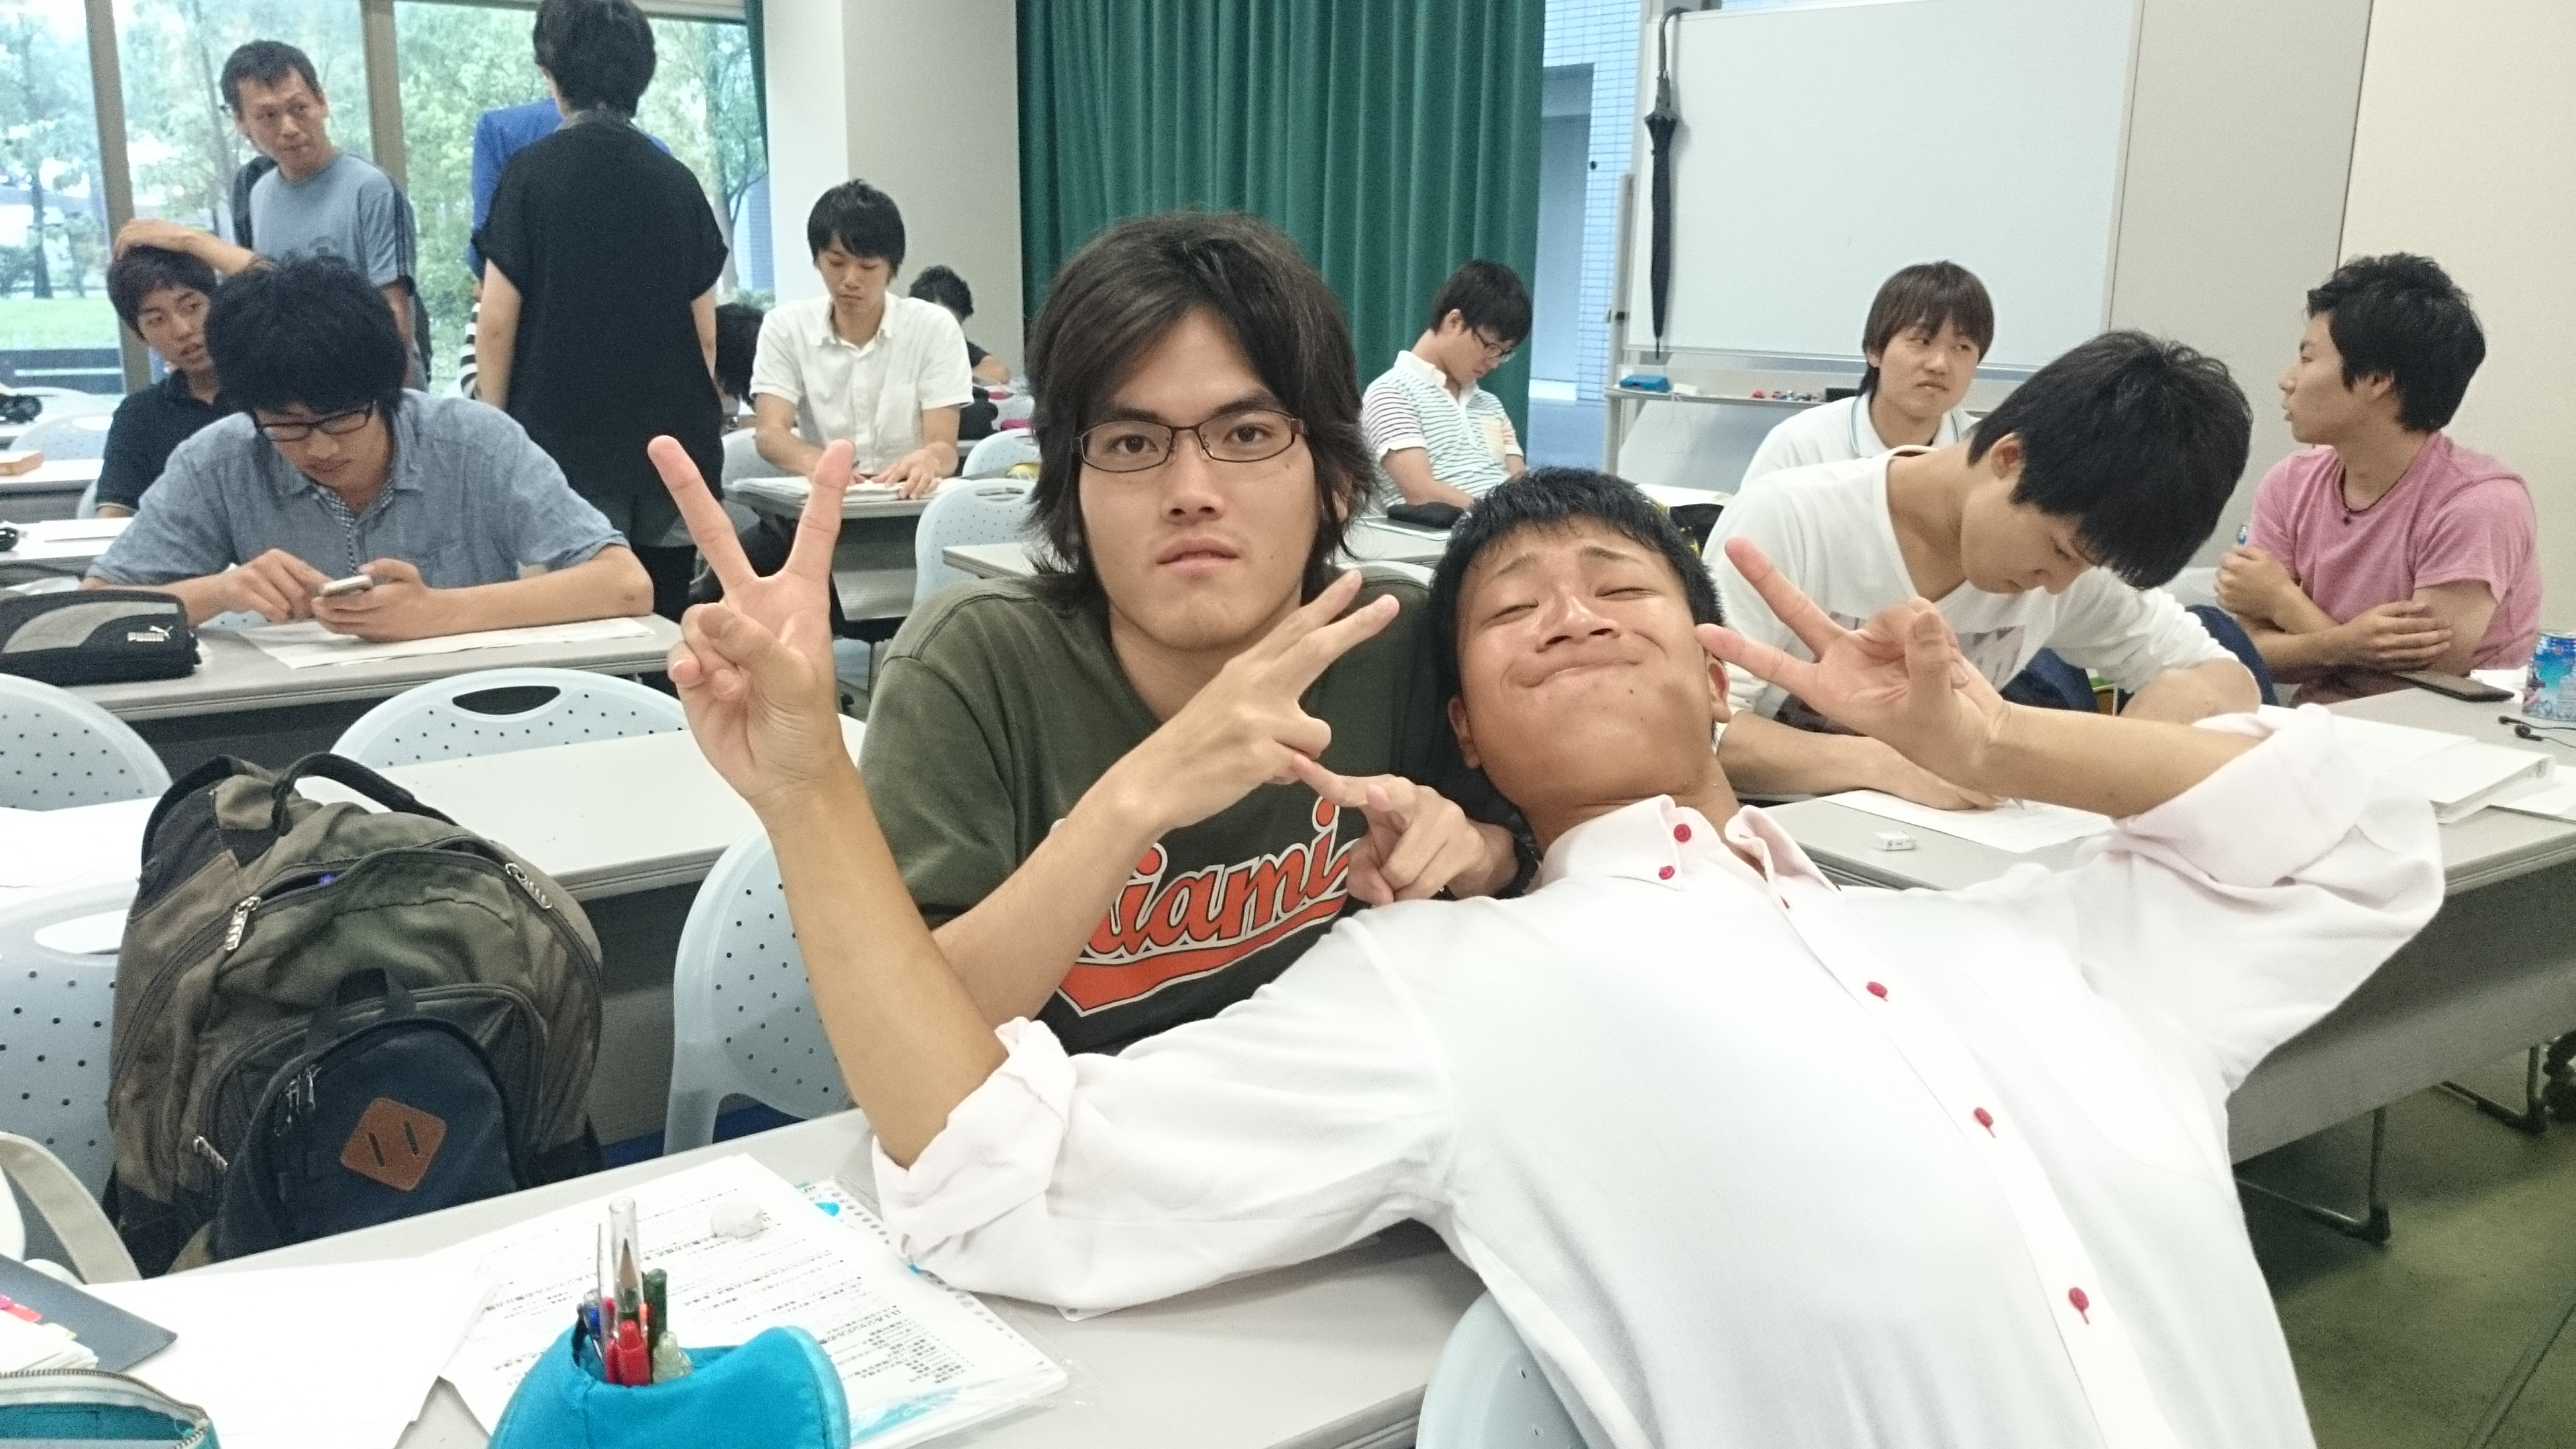
\includegraphics[width=0.8\textwidth]{./section/HigengoUniv/figures/DSC_0388_2}
%\caption{マタヨシ清掃員認定試験会場における、学長と清掃員。}
%\end{figure}
%



%%%%%%%%%%%%%%%%%%%%%%%%%%%%%%%%%%%%%%%%%%%%%%%%%%%%%%%%%
%・非言語大学(タケダ)
%・入学要項、学部、学科、求める学生像、科目数、試験内容、スタッフ一覧
%  ・ポ大学について + 入試問題
% ・非言語大学入試問題について、数学・物理・外国語
%  ・結論:受験生に向けて
